\documentclass{article}

% Language setting
% Replace `english' with e.g. `spanish' to change the document language
\usepackage[english]{babel}

% Set page size and margins
% Replace `letterpaper' with`a4paper' for UK/EU standard size
\usepackage[letterpaper,top=2cm,bottom=2cm,left=3cm,right=3cm,marginparwidth=1.75cm]{geometry}

% Useful packageshttps://www.overleaf.com/project/617db8234c85bd8404625de7
\usepackage{amsmath}
\usepackage{graphicx}
\usepackage{amsthm}
\usepackage{amssymb}
\usepackage[colorlinks=true, allcolors=blue]{hyperref}
\usepackage[dvipsnames]{xcolor}
\newtheorem{theorem}{Theorem}[section]
\newtheorem{corollary}{Corollary}[theorem]
\newtheorem{lemma}[theorem]{Lemma}
\usepackage{float}

\theoremstyle{definition}
\newtheorem{definition}{Definition}[section]

\theoremstyle{remark}
\newtheorem*{remark}{\textbf{Remark}}

\title{MST-311 Final Project}
\author{Rickey Huang, Zhanyang Sun, Lyle Huang}

\newcommand{\qedwhite}{\hfill \ensuremath{\Box}}

\begin{document}
\maketitle

\section{Introduction}

\paragraph{  }

The goal of this project is to first prove the Existence and Uniqueness Theorem for solutions of ordinary differential equations in the form of $\tfrac{\,dy}{\,dt} = f(t,y), y(0) = y_0$. The theorem will be proved in $\mathbb{R}$ first, and it will be stated and proved again in a general metric space defined as $(X,d)$.

\section{The Existence and Uniqueness Theorem in $\mathbb{R}$}

\begin{definition}[\textbf{Lipschitz Function}]\label{def:Lip}
    A function $f(x)$ is a \textbf{Lipschitz Function} if and only if 
    \begin{equation}\label{eqn:Lip}
        \lvert f(x) - f(y) \rvert \leq c \lvert x - y \rvert \;\;\; \text{for all $x, y$, and for some constant $c \in \mathbb{R}$}.
    \end{equation}
    In the other word, the first derivative of $f(x)$ is bounded.
\end{definition}
 
\begin{theorem}[\textbf{The Existence and Uniqueness Theorem in $\mathbb{R}$}]
\label{thm:EUT}
Let $y$ be a \textbf{Lipschitz Function} that continuous in the rectangle $R = \{(t,y)|a < t < b, c < y < d\}$ which contains the point $(0, y_0)$. Then the initial problem
    \begin{equation}\label{eqn:ode}
        \dfrac{\,dy}{\,dt} = f(t,y),\; y(0) = y_0
    \end{equation}
has a unique solution in some interval $I = [-h, h]$, where h is a positive number.
\end{theorem}

\section{The proof to Theorem \ref{thm:EUT}}

\paragraph{  }

The main idea of the proof is followed from the \textbf{Picard Iteration} described in the Section $13.1$ and $13.2$ of the book \textit{Fundamentals of Differential Equations and Boundary Value Problems ($6^{th}$ Edition)} \cite{r_kent_nagle_fundamentals_2011}. The way we prove Theorem \ref{thm:EUT} is to build up a sequence of \textbf{successive approximations} from the differential equation, and we claim that this sequence converges to a unique solution of the differential equation.

\subsection{Converting the Differential Equation into an Integral Equation}

\paragraph{  }

Since we want to get a solution to the function $y$, it is a spontaneous step to take the integral of the differential equation to separate $y$. Thus, we get the following equation by take the integral of the both sides of equation (\ref{eqn:ode}) with lower and upper bounds of $t_0 = 0$ and $t$ separately:

\begin{equation}\label{eqn:integralEqn}
    y(t) = y_0 + \int_{0}^{t} f(s,y(s))\,ds
\end{equation}

\paragraph{  }

We claim that the equation (\ref{eqn:ode}) and equation (\ref{eqn:integralEqn}) are equivalent to each other in the way that they have the same solution. 

\begin{proof}
    First, the solution to equation (\ref{eqn:ode}) also satisfies the equation (\ref{eqn:integralEqn}), since by integrating both sides of the equation (\ref{eqn:ode}), we have 
    \begin{equation}
        \int_{0}^{t}y'(s)\,ds = y(t) - y(0) = \int_{0}^{t} f(s,y(s)) \,ds
    \end{equation}
    Thus, the solution of the original equation should still be the solution to the equation after derivation.
    Conversely, since the function $y$ and $f$ are Lipschitz, they are continuous, hence the solution to the equation (\ref{eqn:integralEqn}) is also the solution to the equation (\ref{eqn:ode}) by differentiating both sides of the equation (\ref{eqn:integralEqn}) using the Fundamental Theorem of Calculus
    \begin{equation}
        \dfrac{d}{\,dt}{(y(t))} = \dfrac{d}{\,dt}{(y_0 + \int_{0}^{t}{f(s,y(s))\,ds})}\\
        \Rightarrow \dfrac{\,dy}{\,dt} = 0 + f(t,y(t)) - 0 = f(t,y(t))
    \end{equation}
    Using this derivation, the solution to the integral equation should also be the solution to the equation (\ref{eqn:ode}). Hence, both equations are equivalent up to the solutions.
\end{proof}

\subsection{Define an Operator to the Solution}

\paragraph{  }

Since we want to construct a sequence of functions that converges to the real solution of the equation (\ref{eqn:ode}), the real solution and the equation we used to approximate should be labelled separately. We use $y$ to denote the real solution and use $\hat{y}$ to indicate the functions that we use to approximate. Then, we use the following equation (\ref{eqn:yhat}) to express $\hat{y}$:

\begin{equation}\label{eqn:yhat}
    \hat{y}(t) = F(y(t)) = y_0 + \int_{0}^{t}{f(s,y(s))}\,ds
\end{equation}

We define an \textbf{operator} to be a mapping that sends a function to a function. In particular, in this case, $F$ is an operator that creates a mapping from $y(x)$ to $\hat{y}(x)$.

\paragraph{  }

In this way, we convert the problem in the equation (\ref{eqn:integralEqn}) to a question of solving the equation (\ref{eqn:operatorEqn}):

\begin{equation}\label{eqn:operatorEqn}
    y(t) = y_0 + \int_{0}^{t}{f(s,y(s))}\,ds = \hat{y}(t) = F(y(t))
\end{equation}

\subsection{Banach Fixed Point Theorem for Functions}

\begin{definition}[\textbf{The Method of Successive Substitution}]\label{def:MethodSS}
The method of \textbf{successive substitution} is a procedure that approaches the fixed point of a function by using the function $f(x)$ in a recursive way. 
\begin{figure}[H]
    \centering
    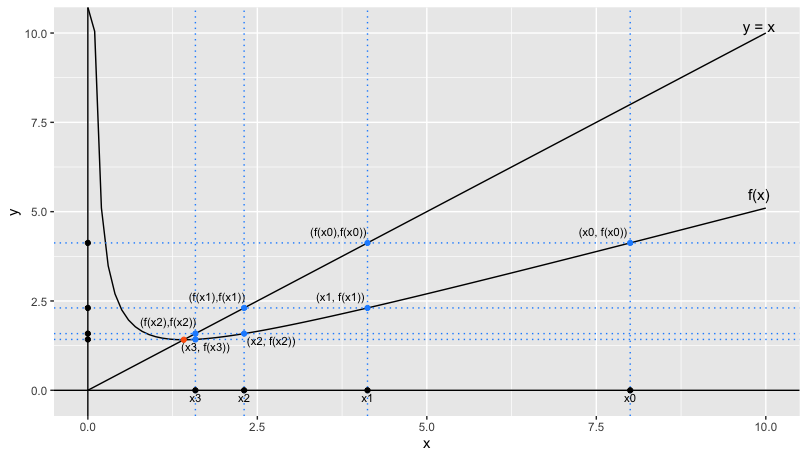
\includegraphics[width=0.8\textwidth]{Successive Approximation Visualization.png}
    \caption{\label{vis:V1}The method of successive approximation}
\end{figure}
Investigating the two curves in the Figure \ref{vis:V1}, the method starts by choosing an arbitrary point on $f(x)$, $x_{0}$ on the domain that is defined, and the point has a coordinate $(x_0, f(x_0))$. If $f(x_0) = x_0$ then $(x_0, f(x_0))$ is on the line $y = x$, which means it is the fixed point of $f(x)$. Then, we are done. Otherwise, if $f(x_0) \neq x_0$, then it is not the fixed point. But if we make a horizontal line through $(x_0,f(x_0))$, it will intersect $y = x$ at $(f(x_0),f(x_0))$, and then make a vertical line through $(f(x_0),f(x_0))$ which intersects $f(x)$ at $(x_1,f(x_1))$. Since $(f(x_0),f(x_0))$ and $(x_1,f(x_1))$ are on the same vertical line, then $x_1 = f(x_0)$. In this way, we create a point that is closer to the fixed point that we want to approach (this conclusion will be justified). Repeating this process we have a $x_2 = f(x_1)$, $\cdots, x_n = f(x_{n-1})$. Hence, we construct a sequence of approximations $\{x_n\}_{n=0}^{\infty}$. If we could prove this sequence converges to some some number, then the fixed point of this function exist. In general, the key idea we used to iterate is the following equation (\ref{eqn:ss}).

\begin{equation} \label{eqn:ss}
    x_{n+1} = f(x_{n})
\end{equation}

\end{definition}

\paragraph{  }

With the help of the method of successive substitution, the following theorem could be introduced.

\begin{theorem}[\textbf{Banach Fixed Point Theorem}]\label{thm:BFPT}
Suppose $g$ is a differentiable function on the closed interval $I$ and $g(x)$ lies in $I$ for all $x$ in $I$. If there exists a constant $K$ such that $\lvert g'(x) \rvert \leq K < 1$ for all $x$ in $I$, then the equation $x = g(x)$ has a unique solution in $I$. Moreover, the sequence of successive approximations defined by 
\begin{equation}\label{eqn:BFPT_sa}
    x_{n+1} = g(x_n), \; n = 0, 1, 2, \cdots
\end{equation}
converges to this solution for any choice of the starting value $x_0$ in $I$.
\end{theorem}

\begin{proof}
    $(1)$ NTS: $\{x_n\}_{n = 1}^{\infty}$ is well defined. \; We will show this using induction. Base case: By hypothesis, we know that $x_0 \in I$. Then, $x_1 = g(x_0) \in I$ since $g(x)$ lies in $I$ for all $x$ in $I$. Inductive hypothesis: Suppose $x_k \in I$, it suffices to show $x_{k+1} \in I$. Inductive step: $x_{k+1} = g(x_k) \in I$, since $g(x)$ is well-defined in $I$. Then by induction for all $n \in \mathbb{N}$ $\{x_n\}_{n = 1}^{\infty}$ is well-defined.
    
    $(2)$ NTS: $\{x_n\}_{n = 1}^{\infty}$ converges to an element in $I$. \; Let $x_m = S_m = x_0 + (x_1 - x_0) + (x_2 - x_1) + \cdots + (x_m - x_{m-1})$. In order to show $\{x_n\}_{n = 1}^{\infty}$ converges, it suffices to show the partial sum $\{S_n\}_{n = 1}^{\infty}$ converges. We will show this partial sum sequence converges using the comparison test and the absolute convergence theorem. First, by mean value theorem, let $p$ and $q$ be two numbers in $I$, then $\exists r \in (p,q) \in I$ such that
    \begin{equation}\label{eqn:MVT}
        g(p) - g(q) = g'(r)(p - q)
    \end{equation}
    Then, since we know 
    \begin{equation}\label{eqn:derivativeBdd}
        \lvert g'(r) \rvert \leq K < 1 \;\;\; \forall r \in I
    \end{equation}
    by assumption, by multiplying $\lvert p - q \rvert$ on the both sides of equation (\ref{eqn:derivativeBdd}), we obtain 
    \begin{equation}\label{eqn:a}
        \lvert g'(r)(p-q) \rvert \leq K \lvert p - q \rvert \;\;\; (K < 1)
    \end{equation}
    Then, by substituting equation (\ref{eqn:MVT}) into the equation (\ref{eqn:a}), we have 
    \begin{equation}\label{eqn:bddLink}
        \lvert g(p) - g(q) \rvert \leq K \lvert p - q \rvert
    \end{equation}
    We will show the sequence $\{S_n\}_{n = 1}^{\infty}$ converges absolutely by proving each increment in the partial sum is bounded. In other words, we will show $\lvert x_{m+1} - x_{m}\rvert$ is bounded by induction. Base case: Notice, the equation (\ref{eqn:bddLink}) applies for all $p$ and $q$ in I. Then, in particular, $\lvert x_2 - x_1 \rvert = \lvert g(x_1) - g(x_0) \rvert \leq K \lvert x_1 - x_0 \rvert$. Hence $\lvert x_2 - x_1 \rvert$ is bounded. Inductive hypothesis: Suppose, $\lvert x_{l} - x_{l-1} \rvert$ is bounded by $K^{l-1} \rvert x_1 - x_0 \rvert$; i.e. $\lvert x_{l} - x_{l-1} \rvert \leq K^{l-1} \rvert x_1 - x_0 \rvert$. Inductive step: It remains to show $\lvert x_{l+1} - x_{l} \rvert \leq K^{l} \rvert x_1 - x_0 \rvert$. Indeed, since $\rvert x_{l + 1} - x_l \rvert = \lvert g(x_l) - g(x_{l-1}) \rvert$, then by the equation (\ref{eqn:bddLink}) and the inductive hypothesis, we have
    \begin{equation}
        \rvert x_{l + 1} - x_l \rvert = \lvert g(x_l) - g(x_{l-1}) \rvert \leq K \lvert x_l - x_{l-1}\rvert \leq K \cdot K^{l-1} \rvert x_1 - x_0 \rvert
    \end{equation}
    Hence, we have $\lvert x_{l+1} - x_l \rvert \leq K^l \lvert x_1 - x_0 \rvert \; (K < 1)$. Thus, by induction, we proved that $\lvert x_{m+1} - x_m \rvert \leq K^m \lvert x_1 - x_0 \rvert \; \forall m \in \mathbb{N} \; (K < 1)$. Then 
    \begin{equation}\label{eqn:comparison}
        \sum_{n = 0}^{\infty}{\lvert x_{n+1} - x_n \rvert} \leq \sum_{n = 0}^{\infty}{K^n\lvert x_1 - x_0 \rvert} = \lvert x_1 - x_0 \rvert \sum_{n = 0}^{\infty}{K^n} \; (K < 1)
    \end{equation}
    Thus, since the sequence $\lvert x_1 - x_0 \rvert \sum_{n = 0}^{\infty}{K^n}$ converges to $\lvert x_1 - x_0 \rvert \cdot \tfrac{1}{1-K}$ (notice, $\sum_{n = 0}^{\infty}{K^n}$ is a geometric series with $K < 1$). Then, by the comparison test, we know $\sum_{n = 0}^{\infty}{\lvert x_{n+1} - x_n \rvert}$ converges. Finally, by absolute convergence theorem, we know $\sum_{n = 0}^{\infty}{x_{n+1} - x_n}$ converges, therefore $\{S_n\}_{n = 1}^{\infty} = \{x_0 + \sum_{n = 0}^{\infty}{x_{n+1} - x_n}\}_{n = 1}^{\infty}$ converges. Hence $\{x_n\}_{n = 1}^{\infty}$ converges. Let $x^{*} := \lim_{n \to \infty}{x_n}$, then $x^{*} \in I$, since $I$ is closed.
    
    $(3)$ NTS: $x^{*}$ is a fixed point of function $g(x)$. \; Since $g(x)$ is continuous, then
    \begin{equation}
        x^{*} = \lim_{n\to \infty}{x_{n+1}} = \lim_{n \to \infty}{g(x_n)} = g(\lim_{x \to \infty}{x_n}) = g(x^{*})
    \end{equation}
    Thus, $x^{*}$ is a fixed point of $g(x)$.
    
    $(4)$ NTS: the fixed point $x^{*}$ is unique in $I$. \; We will show this by contradiction. Suppose by contradiction that there is another fixed point $y$ that is different from $x^{*}$, i.e. $y = g(y)$. Then, from the equation (\ref{eqn:bddLink}), we have
    \begin{equation}
        \lvert x^{*} - y \rvert = \lvert g(x^{*}) - g(y) \rvert \leq K \lvert x^{*} - y \rvert \Rightarrow (1-K)\lvert x^{*} - y \rvert \leq 0
    \end{equation}
    Since $K < 1$, then $1 - K > 0$, and $\lvert x^{*} - y \rvert$ is non-negative, then $(1-K)\lvert x^{*} - y \rvert$ is non-negative. This forces $(1-K)\lvert x^{*} - y \rvert = 0$, therefore $\lvert x^{*} - y = 0$. Hence $x^{*} = y$, which is a contradiction, since we assume $x^{*}$ and $y$ distinct. Therefore, $x^{*}$ is unique in $I$.
\end{proof}

\subsection{Banach Fixed Point Theorem for Operators}

\paragraph{  }

Consider the equation (\ref{eqn:operatorEqn}), the solution we want to find is where the input and the image of the operator $F$ meet each other. We define this intersection of the input and output as the \textbf{fixed point} of the operator $F$. 

\begin{remark}

We generalize the notion of the fixed point for functions. The \textbf{fixed point of a function} is a point that has the same $x$ and $y$ values, which is the intersection between the function and the line $y = x$. Here we are considering the \textbf{fixed point of an operator} of functions by finding, similarly, a function that maps to itself by applying the operator on it. In an other word, it is the intersection between the operator we have and the the operator $T(y(x)) = y(x)$

\end{remark}

\paragraph{  }

Extending from the case of function to operators, we could apply the definition \ref{def:MethodSS} to the operator case. We could follow the same mindset in the previous definition, but the only things different are that first, the operator is playing the role of the function in the definition \ref{def:MethodSS}, while the points that we iterated in the previous definition are corresponding to the functions in the new definition for operator.

\begin{definition}[\textbf{The Method of Successive Approximation for Operators}]\label{def:methodSSO}

Similar to the definition \ref{def:MethodSS}, if there is a fixed point $y(x)$ for the operator $F(y(x))$, we could construct a sequence of approximations of functions $\{y_n(x)\}_{n=0}^{\infty}$ that converges to the fixed point of the operator. We describe this recursive procedure using an equation similar to the equation (\ref{eqn:ss}):

\begin{equation}\label{eqn:sso}
    y_{n+1}(x) = F(y_n(x))
\end{equation}

The equation (\ref{eqn:sso}) is also called as the \textbf{Picard's Iteration}.

\end{definition}

\begin{definition}[\textbf{uniform convergence}]\label{def:uniConv}

A sequence of function $\{y_n(x)\}_{n = 0}^{\infty}$ defined on $C[a,b] \in \mathbb{R}$ converges uniformly to $y(x)$ if and only if $\forall \epsilon > 0, \exists N(\epsilon) \in \mathbb{N}$, such that $\forall n > N, {\lvert\lvert(y_n(x) - y(x)\rvert\rvert} < \epsilon$. i.e. 

\begin{equation}
    \lim_{n \to \infty}{\lvert\lvert y_n(x) - y(x) \rvert\rvert} = \lim_{n \to \infty}{max_{[a,b]}{\lvert y_n(x)-y(x)\rvert}} = 0
\end{equation}
Denoted as $y_n(x) \xrightarrow{unif} y(x)$.
\end{definition}

\paragraph{  }

Using this definition, a stronger version of Banach Fixed Point Theorem will be defined as the following:

\begin{theorem}[\textbf{Banach Fixed Point Theorem for Operators}]\label{thm:BFPTO}
    Let $S$ denote the set of continuous functions on $[a,b]$; i.e.
    \begin{equation}
        S = \{y\in C[a,b]:\lvert\lvert y - y_0\rvert\rvert \leq \alpha\}
    \end{equation}
    for some $a, b, \alpha\in \mathbb{R}$. Suppose $T$ is an operator mapping S into $S$ and that $T$ is a \textbf{contraction} on $S$, which means that there exist a constant $K$, $0\leq K < 1$, such that 
\begin{equation}\label{eqn:contractionO}
    \lvert\lvert T(w) - T(z) \rvert\rvert \leq K\lvert\lvert w - z \rvert\rvert \text{ for all } w,z \text{ in } S \text{.}
\end{equation}
Then the equation $y = F(y)$ has a unique solution in $S$. Moreover, the sequence of successive approximation given by
\begin{equation}\label{eqn:ssoex}
    y_{n+1} = T(y_n), \; \; \; n = 0, 1, 2, \cdots,
\end{equation}
converges uniformly to this solution for any choice of the starting function $y_0$ in $S$.
\end{theorem}

\begin{proof}
    $(1)$ NTS: $\{y_n\}_{n = 1}^{\infty}$ is well defined. \; We will show this using induction. By hypothesis, we know that $y_0 \in S$. Then, $y_1 = T(y_0) \in S$ since $T(y)$ lies in $S$ for all $y$ in $S$. Then by induction for all $n \in \mathbb{N}$, $y_n = T(y_{n-1}) \in S$, so that $\{x_n\}_{n = 1}^{\infty}$ is well-defined.
    
    $(2)$ NTS: $\{y_n\}_{n = 1}^{\infty}$ converges to an element in $S$. \; Let $y_m = S_m = y_0 + \sum_{n = 0}^{m}(y_{n+1} - y_n)$. In order to show $\{y_n\}_{n = 1}^{\infty}$ converges, it suffices to show the partial sum $\{S_n\}_{n = 1}^{\infty}$ converges. We will show this partial sum sequence converges using the Weierstrass M-test. First, each increment in the partial sum can be proved to be bounded using the contraction assumption by induction. In other words, $\lvert\lvert y_{m+1} - y_{m}\rvert\rvert$ is bounded by induction. Notice, the equation (\ref{eqn:contractionO}) applies for all $w$ and $z$ in $S$. In particular, $\lvert\lvert y_2 - y_1 \rvert\rvert = \lvert\lvert T(y_1) - T(y_0) \rvert\rvert \leq K \lvert\lvert y_1 - y_0 \rvert\rvert$. Hence, $\lvert\lvert x_2 - x_1 \rvert\rvert$ is bounded by $K \lvert\lvert y_1 - y_0 \rvert\rvert$. By induction,
    \begin{equation}
        \lvert\lvert y_{m+1} - y_{m} \rvert\rvert \leq K \lvert\lvert y_m - y_{m-1} \rvert\rvert \leq K^2 \lvert\lvert y_{m-1} - y_{m-2} \rvert\rvert \leq \cdots \leq K^m\lvert\lvert y_1 - y_0 \rvert\rvert \; \forall m \in \mathbb{N} \; (K < 1)
    \end{equation}
   Then because we define $\lvert\lvert * \rvert\rvert = max_{[a,b]}\lvert * \rvert \in \mathbb{R}$,
    \begin{equation}\label{eqn:comparison}
        \sum_{n = 0}^{\infty}{\lvert y_{n+1} - y_n \rvert} \leq \sum_{n = 0}^{\infty}{K^n\lvert y_1 - y_0 \rvert} = \lvert y_1 - y_0 \rvert \sum_{n = 0}^{\infty}{K^n} \; (K < 1)
    \end{equation}
    Thus, the sequence $\lvert y_1 - y_0 \rvert \sum_{n = 0}^{\infty}{K^n} = \lvert y_1 - y_0 \rvert \cdot \tfrac{1}{1-K}$ (notice, $\sum_{n = 0}^{\infty}{K^n}$ is a geometric series with $K < 1$). Then, by the Weierstrass M-test, we know $\sum_{n = 0}^{\infty}{y_{n+1} - y_n}$ converges uniformly on $C[a,b]$. Hence $\{y_n\}_{n = 1}^{\infty}$ converges uniformly. Let $y^{*} := \lim_{n \to \infty}{y_n}$, then since $y^{*} \in C[a,b]$, $y^{*} \in S$.
    
    $(3)$ NTS: $y^{*}$ is a fixed point of function $T(y)$. \; Let $\epsilon > 0$, $\exists N \in \mathbb{N}$, such that $\forall n > N, \lvert\lvert y_n - y^{*} < \epsilon$ because $y_n \xrightarrow{unif} y^{*}$. We will show $\forall n > N, \lvert\lvert T(y_n) - T(y^{*}) \rvert\rvert < \epsilon$. Indeed, using the contraction map,
    \begin{equation}
        \lvert\lvert T(y_n) - T(y^{*}) \rvert\rvert \leq K \lvert\lvert y_n - y^{*} \rvert\rvert < \epsilon
    \end{equation}
    Hence $T(y_n) \xrightarrow{unif} T(y^{*})$. Also, we know $T(y_n) = y_{n+1} \xrightarrow{unif} y^{*}$. Then, since the limit is unique, $T(y^{*}) = y^{*}$. Thus, $y^{*}$ is a fixed point of $T(y)$.
    
    $(4)$ NTS: the fixed point $y^{*}$ is unique in $S$. \; We will show this by contradiction. Suppose by contradiction that there is another fixed point $z$ that is different from $y^{*}$, i.e. $z = T(z)$. Then, from the equation (\ref{eqn:contractionO}), we have
    \begin{equation}
        \lvert\lvert y^{*} - z \rvert\rvert =\lvert\lvert T(y^{*}) - T(z) \rvert\rvert \leq K \lvert\lvert y^{*} - z \rvert\rvert \Rightarrow (1-K)\lvert\lvert y^{*} - z \rvert\rvert \leq 0
    \end{equation}
    Since $K < 1$, then $1 - K > 0$, and $\lvert\lvert y^{*} - z \rvert\rvert$ is non-negative, then $(1-K)\lvert\lvert y^{*} - z \rvert\rvert$ is non-negative. This forces $(1-K)\lvert\lvert y^{*} - z \rvert\rvert = 0$, therefore $\lvert\lvert y^{*} - z\rvert\rvert = 0$. Hence $y^{*} = z$, which is a contradiction, since we assume $y^{*}$ and $z$ distinct. Therefore, $y^{*}$ is unique in $S$.
\end{proof}

\subsection{Applying Theorem \ref{thm:BFPTO} to prove Theorem \ref{thm:EUT}}

\paragraph{  }

\textcolor{red}{The main idea of this proof is to apply the Theorem \ref{thm:BFPTO} on the equation (\ref{eqn:integralEqn}), $\hat{y}(t) = F(y(t)) = y_0 + \int_{0}^{t}{f(s,y(s))}\,ds$ to prove that the operator $F$ has a fixed point, and this fixed point is the unique solution to the ordinary differential equation in the equation (\ref{eqn:ode}). There are two main assumptions in this theorem: }

$(1)$ We need to define a continuous interval for $\hat{y}(t) = y_0 + \int_{0}^{t}{f(s,y(s))}\,ds$.

$(2)$ We need to show that $F(y)$ is a contraction.

\paragraph{  }

The first assumption is fulfilled by constructing a rectangle $R'$ using two constant $h_1$ and $\alpha_1$ such that it is contained in $R$:
\begin{equation}\label{eqn:rect}
    R' = \{(t,y): \lvert t \rvert \leq h_1, \lvert y - y_0 \rvert \leq \alpha_1\}
\end{equation}

\paragraph{  }

Then, there exists a bound $M > 0$ such that for all $t, y \in R_1$, $\lvert f(x,y) \rvert \leq M$. Since $y(t)$ is a Lipschitz Function, $\exists \; c \in \mathbb{R}$ such that $\lvert y(t_1) - y(t_2) \rvert \leq c \lvert t_1 - t_2 \rvert$ for all $t_1, t_2$. In order to keep the solution in the rectangle, we will choose $h$, such that $0< h < min\{h_1,\tfrac{\alpha_1}{M}, \tfrac{1}{c}\}$, and this $h$ will be used to construct the interval $I = [-h,h]$, where the solution to the ordinary differential equation falls into.

\paragraph{  }

Second, we will show that the $F$ is a contraction on $S$ by showing that 

\begin{align}
        \lvert F(u(t)) - F(v(t)) \rvert & = \lvert \int_{0}^{t}{(y(s,u(s)) - y(s,v(s))) \,ds} \rvert\\
        & \leq c\lvert \int_{0}^{t}{\lvert u(s) - v(s) \rvert \,ds}\rvert\\
        & \leq c\lvert\lvert u - v \rvert\rvert_{I}\lvert t \rvert \leq ch\lvert\lvert u - v \rvert\rvert_{I}
\end{align}

\paragraph{  }

If we set $K = ch$, we have the following equation:

\begin{equation}\label{eqn:contractionI}
    \lvert\lvert F(u) - F(v)\rvert\rvert_{I} \leq K \lvert\lvert u - v \rvert\rvert_{I}
\end{equation}

Also, since we pick $h \leq 1/L$, then $K < 1$. Therefore we prove that F is a contraction.

\subsection{The Existence and Uniqueness Theorem in a General Metric Space $(X,d)$}

\begin{definition}[\textbf{Metric Space}]\label{def:matricSpace}

A \textbf{metric space} $(X,d)$ satisfies the below three properties $\forall x,y \in X$ 
\begin{itemize}
    \item $d(x,y) \geq 0$ and $d(x,y) = 0 \Longleftrightarrow x = y$
    \item $d(x,y) = d(y,x)$
    \item $d(x,z) \leq d(x,y) + d(y,z)$
\end{itemize}

\end{definition}

Basically a metric space defines a distance between the object in a field. with this abstract distance between element in a set defined, we can state a general version of Theorem \ref{thm:EUT} within a general metric space $(X,d)$

\begin{theorem}[\textbf{The Existence and Uniqueness Theorem in $(X,d)$}]\label{thm:EUTXd}
    Let $y$ be a Lipschitz Function that is continuous in the rectangle $R = \{(t,y)|a < t < b, c < y < d\} \subseteq X$ where $a,b,c,d \in X$ and the rectangle contains the point $(0, y_0) \in R \subseteq X$. Then the initial problem
    \begin{equation}
        \dfrac{\,dy}{\,dt} = f(t,y),\; y(0) = y_0
    \end{equation}
has a unique solution in some interval $I = [-h, h]$, where h is an element in $X$.
\end{theorem}

\paragraph{  }

\begin{definition}[\textbf{convergence of a sequence in a metric space $(X,d)$}]\label{def:ConvMetric}
    A sequence $\{x_n\}_{n=1}^{\infty} \subseteq X$ converges to $x \in X$ if and only if $\forall \epsilon > 0, \exists N(\epsilon) \in \mathbb{N}$, such that $\forall n > N, d(x_n - x) < \epsilon$. i.e. 
    \begin{equation}\label{eqn:ConvMetric}
        \lim_{n \to \infty}{d(x_n - x) = 0} \;\;\; \forall n > N
    \end{equation}
\end{definition}

\begin{definition}[\textbf{uniform convergence in a metric space $(X,d)$}]\label{def:uniConvMetric}

    A sequence of function $\{y_n(x)\}_{n = 0}^{\infty}$ defined on $D \subseteq X$ converges uniformly on $D$ to $y(x)$ if and only if $\forall \epsilon > 0, \exists N(\epsilon) \in \mathbb{N}$, such that $\forall n > N, d(y_n(x) - y(x)) < \epsilon$. i.e.
        \begin{equation}
            \lim_{n \to \infty}{d(y_n(x) - y(x))} = 0 \;\;\; \forall n > N
        \end{equation}
    Denoted as $y_n(x) \xrightarrow{unif} y(x)$
\end{definition}

\begin{definition}[\textbf{Cauchy Sequences}]\label{def:cauchySeq}

    A sequence $\{x_n\} \subset X$ is called Cauchy if $d(x_n - x_m) \rightarrow 0$ as $m,n \rightarrow \infty$, i.e. if for any $\epsilon \ \textgreater\ 0$ there is $N = N(\epsilon)$ such that
        \begin{equation}
            \forall\ m,n\ \textgreater\ N \Longrightarrow d(x_n - x_m)\ \textless \ \epsilon
        \end{equation}
\end{definition}

\begin{definition}[\textbf{Completeness}]\label{def:completeness}

    A subset S of X is said to be complete if every Cauchy sequence $\{x_n\} \subset S$ converges to a point $x \in S$
\end{definition}

\begin{theorem}[\textbf{Contraction Mapping theorem}]\label{thm:CMT}
    Let $(X,d)$ be a complete metric space, and $A:X\rightarrow X$ be a contraction mapping. The A has a unique fixed point in X. That is, there is a unique point $x^*\in X$ such that $Ax^* = x^*$. Furthermore, if $x_0$ is any point in X, and define $x_{n+1} = Ax_n$, then $x_n \rightarrow x^*$ as $n \rightarrow \infty$.
\end{theorem}

\newpage

\newpage
\bibliographystyle{alpha}
\bibliography{sources}

\end{document}